\chapter{Accettanza Geometrica di un Rivelatore}\label{ch:acc}
    L'ultima esperienza consiste nel calcolare l'accettanza geometrica di un rivelatore, definita come il rapporto tra il numero di particelle incidenti e il numero di particelle emesse, sfruttando la generazione di numeri casuali e il metodo montecarlo.

    \section{Il sistema fisico proposto}
        L'obiettivo che mi sono posto è stato quello di calcolare l'accettanza geometrica di un rivelatore a forma di dischetto con raggio variabile, posto in una posizione arbitraria nel semispazio positivo delle $z$. Allo stesso modo, la sorgente di particelle è costituita da un secondo dischetto, anch'esso con raggio variabile, centrato nell'origine.

        Le ipotesi che ho fatto sono le seguenti:
        \begin{enumerate}
            \item Ciascun punto della sorgente emette in maniera isotropa, ovvero in tutte le direzioni con la stessa probabilità;
            \item La probabilità di emissione da parte di un punto della sorgente è uniforme, ovvero tutti i punti hanno la stessa probabilità di emettere una particella;
            \item Il rivelatore e la sorgente sono sempre paralleli tra loro e al piano $Oxy$, e il rivelatore è sempre posto sopra la sorgente.
        \end{enumerate}

        Per ragioni di simmetria, la posizione del rivelatore sopra la sorgente non causa alcuna perdita di generalità. Se il rivelatore avesse altezza $z=0$, visto lo spessore nullo sia della sorgente che del rivelatore, nessuna particella verrebbe rivelata. La sorgente inoltre emette in modo simmetrico rispetto al piano $Oxy$, quindi il caso $z<0$ è equivalente al caso $z>0$.

        \subsection{Sorgente puntiforme}\label{ss:acc:sorgente-puntiforme}
            Dal momento che la sorgente può emettere da un solo punto alla volta, cominciamo col risolvere il problema nel caso di una sorgente puntiforme nell'origine e un rivelatore che può essere spostato rispettando le ipotesi di cui sopra. 
            
            Affinché la distribuzione delle particelle sia uniforme, generare delle coordinate cartesiane casuali non è sufficiente. La scelta che ho fatto è quella di generare delle \emph{direzioni} casuali in coordinate sferiche $\pqty{\varrho,\vartheta,\varphi}$, risparmiando la spesa computazionale di generare la distanza $\varrho$ dall'origine. Per le proprietà delle coordinate sferiche possiamo generare uniformemente $\cos\!\vartheta\in\bqty{-1;1}$, per poi ricavare $\vartheta$ prendendone l'arcocoseno, mentre possiamo generare uniformemente $\varphi\in\bqty{0;2\pi}$.

            Fissata una direzione $\pqty{\vartheta,\varphi}$, la particella emessa dalla sorgente si muoverà lungo la retta che passa per l'origine avente tale direzione. Ci chiediamo quindi se questa retta intersecherà il rivelatore, e in caso affermativo, in quale punto.\footnote{Sapere il punto non è necessario per il calcolo dell'accettanza geometrica, ma è utile allo scopo di generare un'immagine del sistema.}

            Da semplici considerazioni geometrice, se indichiamo con $P\equiv\pqty{x,y,z}$ il generico punto dello spazio, con $C\equiv{x_c,y_c,z_c}$ il centro del rivelatore e con $R$ il suo raggio, il punto appartiene al dischetto se si verificano contemporaneamente le seguenti condizioni:
            \begin{align}
                \pqty{P - C}^2 &\leq R^2 \mycomma
                \label{eq:acc:cond-1}
                \\
                z &= z_c \myperiod
                \label{eq:acc:cond-2}
            \end{align}
            La prima condizione corrisponde a $\pqty{x - x_c}^2 + \pqty{y - y_c}^2 + \pqty{z - z_c}^2 \leq R^2$, che messa a sistema con la seconda dà $\pqty{x - x_c}^2 + \pqty{y - y_c}^2 \leq R^2$. Passiamo quindi a coordinate polari per trovare le condizioni che devono rispettare i valori di $\vartheta$ e $\varphi$:
            \begin{equation*}
                \begin{cases}
                    x = \varrho\sin\!\vartheta\cos\!\varphi \\
                    y = \varrho\sin\!\vartheta\sin\!\varphi \\
                    z = \varrho\cos\!\vartheta
                \end{cases}
                \myperiod
            \end{equation*}
            Sostituendo queste relazioni nella condizione di appartenenza al cerchio troviamo:
            \begin{equation*}
                \pqty{\varrho\sin\!\vartheta\cos\!\varphi - x_c}^2 + \pqty{\varrho\sin\!\vartheta\sin\!\varphi - y_c}^2 \leq R^2
                \mycomma
            \end{equation*}
            che con qualche passaggio si riduce a
            \begin{equation*}
               \varrho^2 \sin\!^2\vartheta + x_c^2 + y_c^2 - 2 \varrho\sin\!\vartheta\pqty{x_c\cos\!\varphi + y_c\sin\!\varphi} \leq R^2
               \mycomma
            \end{equation*}
            che a sua volta, a patto di porre $d^2 = x_c^2 + y_c^2$, $x_c = d\cos\!\varphi_c$ e $y_c = d\sin\!\varphi_c$, non è altro che il teorema del coseno applicato al triangolo formato dalle proiezioni sul piano $Oxy$ dei punti $O$, $P$ e $C$, che ha un angolo in $O$ proprio pari a $\varphi - \varphi_c$:
            \begin{equation}
                \varrho^2 \sin\!^2\vartheta + d^2 - 2 \varrho\sin\!\vartheta d \cos\!\pqty{\varphi - \varphi_c} \leq R^2
                \myperiod
                \label{eq:acc:cond-rho}
            \end{equation}
            Se assumiamo $\cos\!\vartheta \neq 0$---che è vero se $P \notin Oxy$, e ciò non è restrittivo in quanto il piano è un sottoinsieme a misura nulla dello spazio $\R^3$---possiamo invertire la \eqref{eq:acc:cond-2} scritta in coordinate polari per esplicitare $\varrho$:
            \begin{equation}
                \varrho = \frac{z_c}{\cos\!\vartheta}
                \myperiod
                \label{eq:acc:rho-expl}
            \end{equation}
            Sostituendo quest'ultima relazione \eqref{eq:acc:rho-expl} nella \eqref{eq:acc:cond-rho} si ottiene
            \begin{equation}
                z_c \tan\!\vartheta + d^2 - 2 z_c \tan\!\vartheta d \cos\!\pqty{\varphi - \varphi_c} \leq R^2
                \myperiod
                \label{eq:acc:diseq}
            \end{equation}

            I valori $z_c$, $d$ e $\varphi_c$ sono costanti, per cui una volta generati $\vartheta$ e $\varphi$ è sufficiente verificare la disequazione per sapere se il raggio interseca o no il rivelatore. Resta quindi da trovare esplicitamente la posizione dei punti $P^*\equiv\pqty{x^*, y^*, z^*}$ che soddisfano la relazione; il problema può essere ridotto a quello dell'intersezione tra la retta individuata dalla direzione $\pqty{\vartheta,\varphi}$ e il piano $z = z_c$. La quantità $z_c \tan\!\vartheta$ è la proiezione del segmento $\overline{OP^*}$ sul piano $Oxy$: il suo prodotto per $\cos\!\varphi$ e $\sin\!\varphi$ ci dà rispettivamente le coordinate $x^*$ e $y^*$. L'altezza $z^*$ è naturalmente la stessa del rivelatore $z_c$.
            
            È importante notare che il problema non distingue tra ``sopra'' e ``sotto'', per cui un raggio rivolto verso il simmetrico di $P^*$ rispetto all'origine sarà ugualmente soluzione della disequazione. Per tener conto di ciò basterà dividere per $2$ il conteggio totale dei punti che intersecano il rivelatore nel calolo dell'accettanza geometrica.

        \subsection{Sorgente estesa}
            Per estendere quanto sviluppato al punto precedente alla sorgente estesa, è sufficiente fare una semplice traslazione: generato un punto $S\equiv\pqty{x_s, y_s, 0}$ arbitrario nella sorgente circolare, è possibile calcolare la posizione relativa del centro $C'$, nel sistema di riferimento che ha il cento in $S$, che avrà quindi coordinate $C'\equiv\pqty{x_c - x_s, y_c - y_s, z_c}$. Fatto ciò possiamo generare una direzione casuale e, con gli stessi passaggi del punto precedente, trovare gli eventuali punti di intersezione nel sistema di riferimento del punto sorgente. Trovati tali punti, sarà immediato riportarli nel sistema di riferimento del centro della sorgente con la traslazione inversa. Si trova in particolare
            \begin{equation*}
                \begin{cases}
                    x^* = x_s + z_c\tan\!\vartheta\cos\!\varphi \\
                    y^* = x_s + z_c\tan\!\vartheta\sin\!\varphi \\
                    z^* = z_c
                \end{cases}
                \mycomma
            \end{equation*}
            dove $\vartheta$ e $\varphi$ sono ancora le direzioni generate casualmente nel sistema del punto sorgente; $z_c$ resta invariato dal momento che il punto $S$ giace ancora in $Oxy$.
    
    \section{Codice e generazione dei punti}
        Come per la simulazione dell'assorbimento di particelle cariche esposto al Capitolo \Sref{ch:bet}, anche per questo progetto l'interezza del codice è reperibile sul mio profilo GitHub.\footnote{Repository: \url{https://github.com/ImAure/geometric-acceptance}}

        Il programma può essere lanciato scegliendo fin da subito il numero di punti da generare, le dimensioni della sorgente e del rivelatore e la posizione di quest'ultimo. Dopo aver verificato la validità dell'input e caricati i dati in memoria, il programma genera un punto casuale come sorgente in coordinate polari piane e una direzione casuale per la radiazione in coordinale polari sferiche.
        \lstinputlisting[style = CStyle]{code/accettanza/random.txt}
        Affinché la distribuzione sia uniforme, nel caso bidimensionale viene generato uniformemente $\varrho^2 \in \bqty{0;1}$, ne viene presa la radice quadrata e il risultato è moltiplicato per il raggio massimo. Nel caso tridimensionale la funzione fa la stessa cosa con $\varrho^3$ e la radice terza, mentre come detto prima viene generato\footnote{Per essere precisi, il coseno è generato tra \num{1} e \num{-1} piuttosto che tra \num{-1} e \num{1}. Questo perché per $\vartheta = 0$ si ha $\cos\!\vartheta = \num{1}$ e per $\vartheta = \pi$ si ha $\cos\!\vartheta = \num{-1}$} $\cos\!\vartheta \in \bqty{-1;1}$ e ne viene preso l'arcocoseno per avere $\vartheta$.

        Entrambe le funzioni ammettono come input anche un raggio massimo negativo: in quel caso il raggio verrà posto uguale a $1$ e verrà generata solo la direzione. Questo comportamento è sfruttato nella generazione casuale della radiazione, in cui la chiamata a funzione avviene come \verb|rand_polar3D(&ray, -1)|.
        
        La funzione \verb|intercept()| verifica l'intersezione del raggio nel caso di una sorgente puntiforme posta nell'origine. Per utilizzarla correttamente viene calcolata la posizione relativa del rivelatore $\pqty{x_c', y_c', z_c}$ e questa viene data in input alla funzione insieme alla direzione da verificare.
        \lstinputlisting[style = CStyle]{code/accettanza/intercept.txt}
        La funzione valuta quindi la disequazione \eqref{eq:acc:diseq} e in caso di successo aggiorna il conteggio e stampa su file le coordinate del punto di partenza e del punto di arrivo, dopo averle riportate di nuovo nel riferimento del centro della sorgente.

        Sullo stesso file, la funzione \verb|intercept()| si occupa anche di stampare la posizione dei punti di intersezione del rivelatore convertendoli in coordinate polari nel sistema di riferimento centrato nel rivelatore stesso. Questi dati possono essere usati per costruire un istogramma e apprezzare la non uniformità della distribuzione della radiazione sul sensore.

        L'accettanza geometrica del rivelatore è infine calcolata dividendo il numero di raggi che intersecano il rivelatore per il numero totale di raggi generati. Come giustificato alla fine del punto \Sref{ss:acc:sorgente-puntiforme}, questo numero è a sua volta diviso per \num{2} per tenere conto solo dei raggi che viaggiano nel semispazio $z > 0$; analogamente anche il numero \verb|hits|, prima di essere stampato a schermo, è diviso per \num{2} e arrotondato. Il programma quindi stampa a schermo anche l'accettanza geometrica del rivelatore e l'equivalente angolo solido che esso sottende.

    \section{Esempi e immagini}
        Riporto qui degli esempi di esecuzione della simulazione. Il nome dell'eseguibile è \verb|sim|, mentre gli argomenti che compaiono sono in ordine il numero di punti da generare, il raggio della sorgente, le coordinate $\pqty{x,y,z}$ del centro del rivelatore e la stringa da usare per i nomi dei file in cui salvare tutti i punti generati, \verb|<string>.1.txt|, e i punti da graficare, \verb|<string>.2.txt|.

        Le immagini sono generate tramite uno script python che estrae i numeri dal secondo file. La prima parte del programma rappresenta i punti di partenza dei raggi in rosso e i punti di arrivo in verde, collegandoli con una riga grigia; la seconda parte del programma crea un istogramma in tre dimensioni i cui bin sono settori di corone circolari. I bin sono generati in modo da avere area costante, per questo quelli più esterni sono più sottili. L'altezza delle barre invece è la densità di frequenza ottenuta dividendo la frequenza relativa per l'area del bin.

        \begin{figure}[ht]
            \textbf{Sorgente piccola e rivelatore allineato}
            \lstinputlisting[style = mybash]{code/accettanza/bash1.txt}
            \centering
            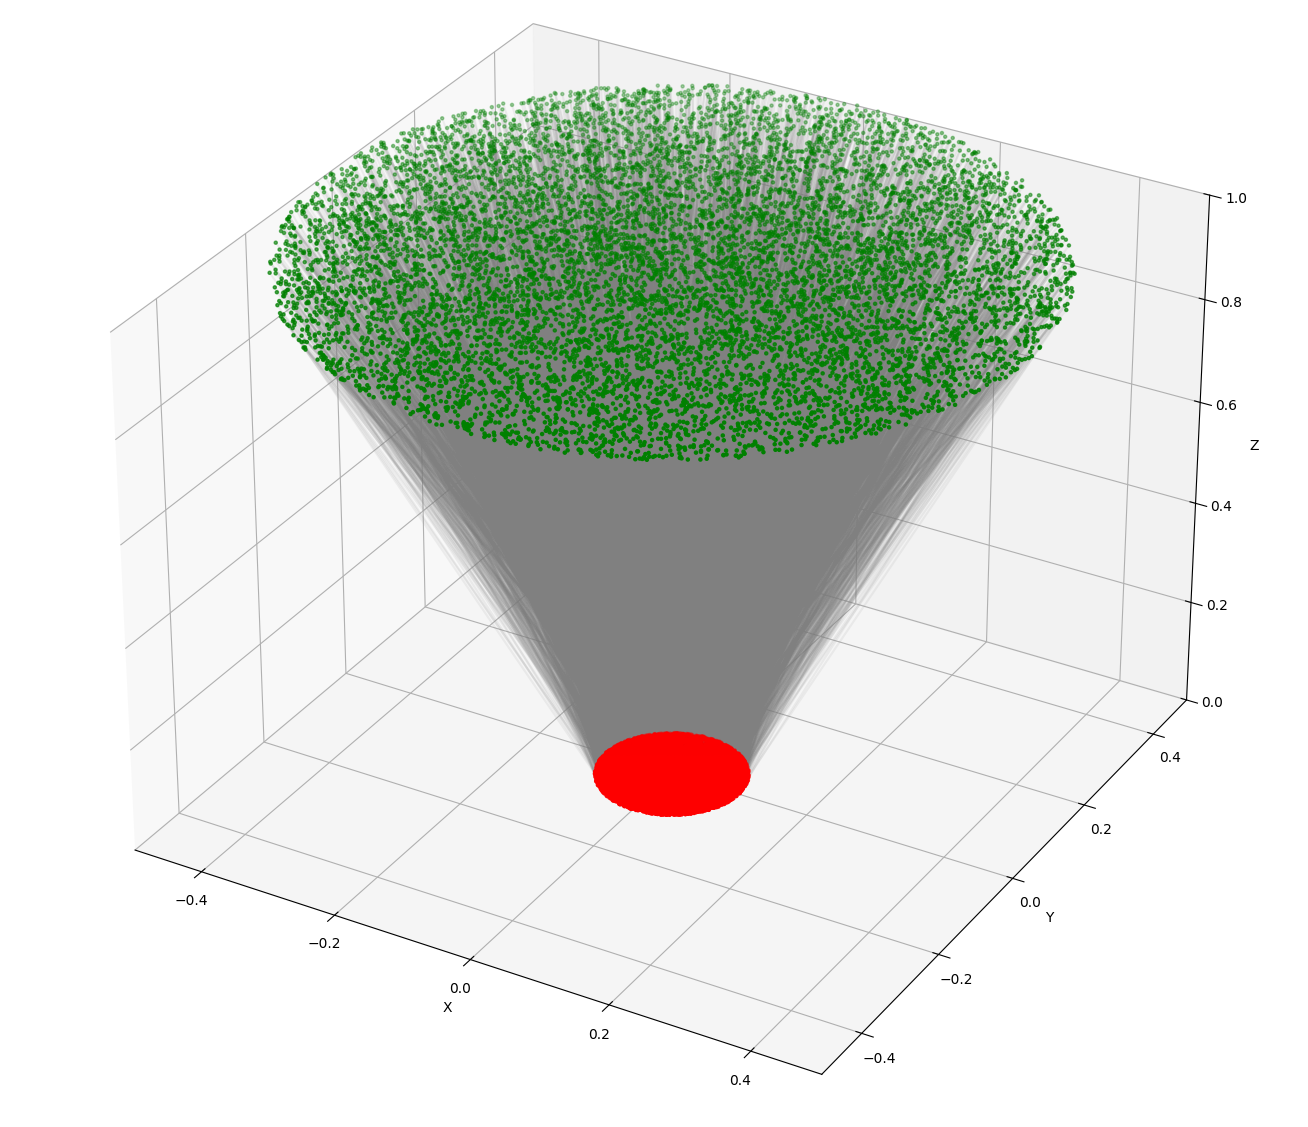
\includegraphics[width=0.49\textwidth]{images/accettanza/example1.1.png}
            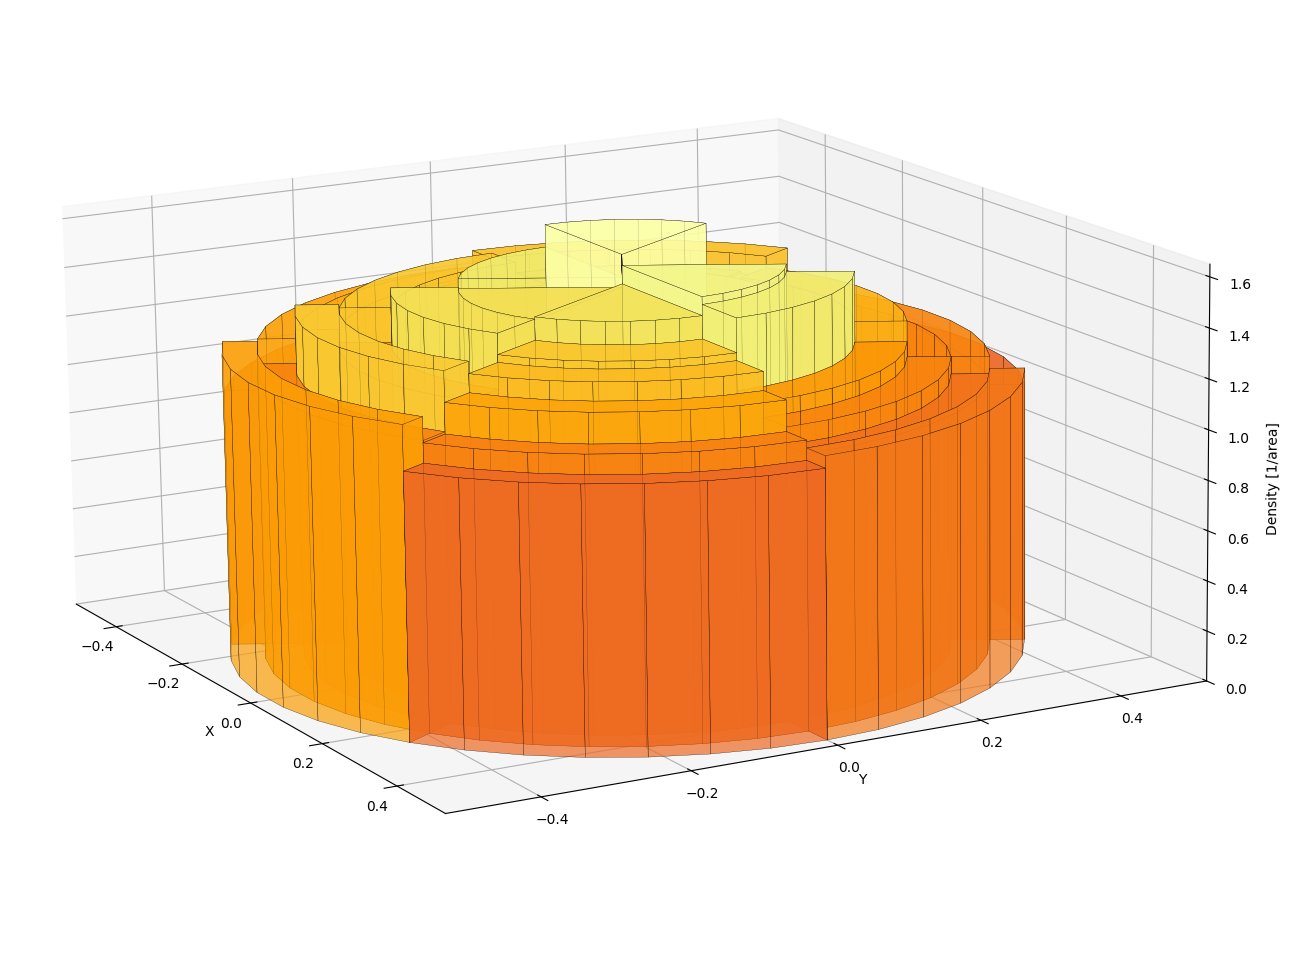
\includegraphics[width=0.49\textwidth]{images/accettanza/example1.2.png}
            \caption{Notiamo dall'istogramma che la distribuzione è maggiormente concentrata al centro.}
        \end{figure}

        \begin{figure}[ht]
            \textbf{Sorgente puntiforme e rivelatore traslato}
            \lstinputlisting[style = mybash]{code/accettanza/bash2.txt}
            \centering
            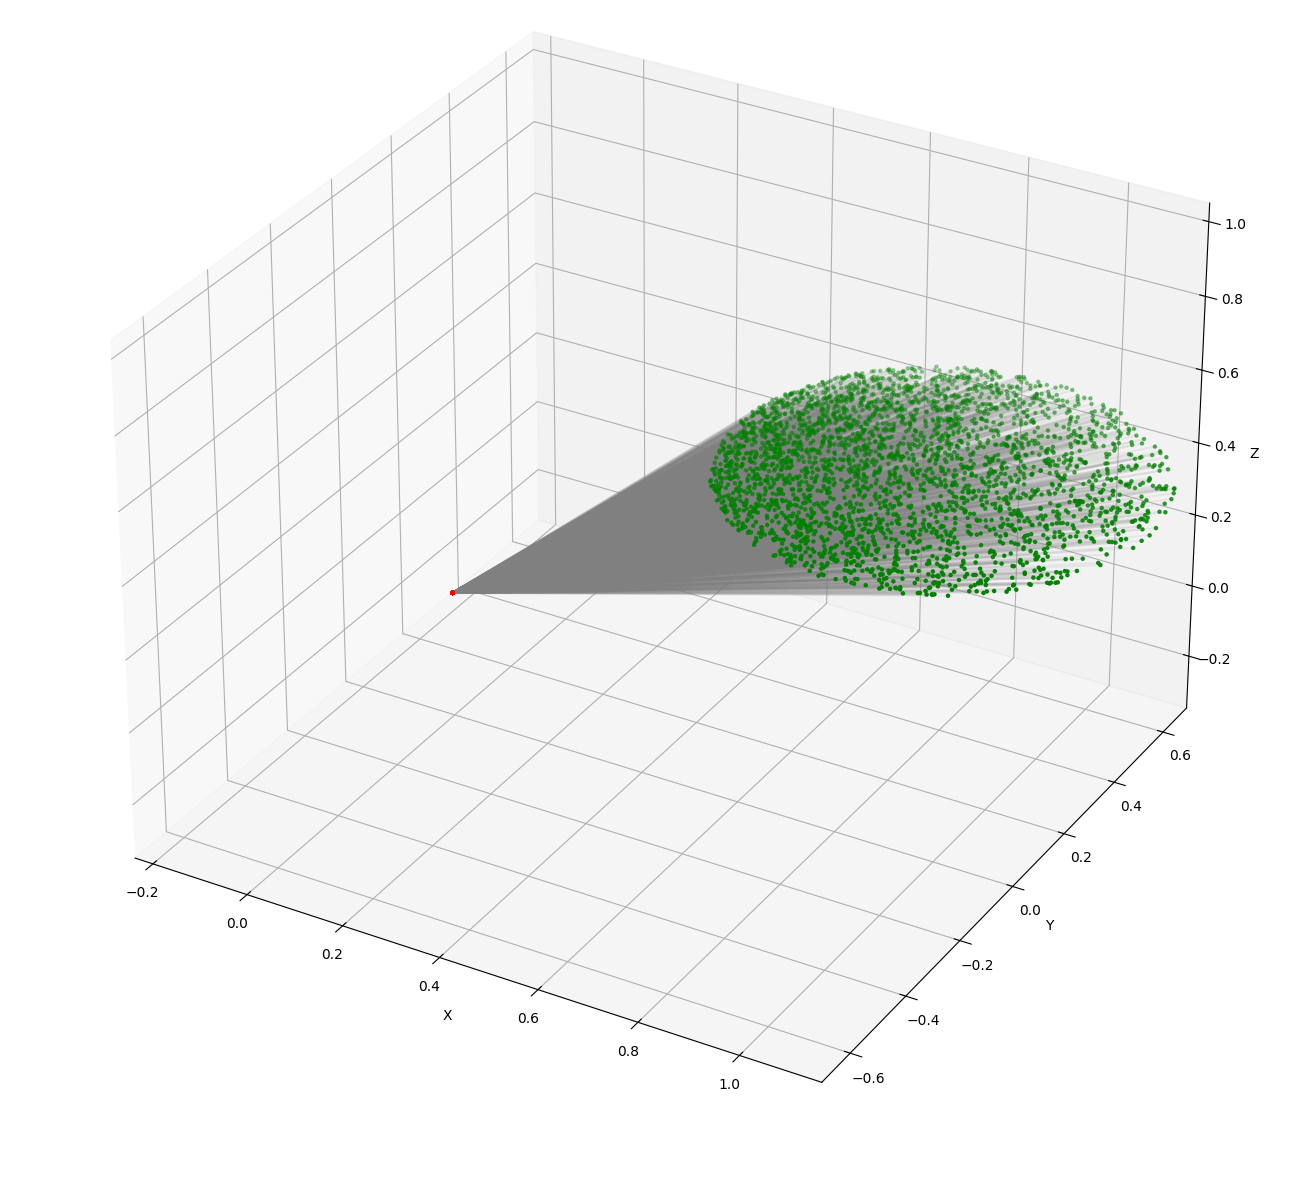
\includegraphics[width=0.49\textwidth]{images/accettanza/example2.1.png}
            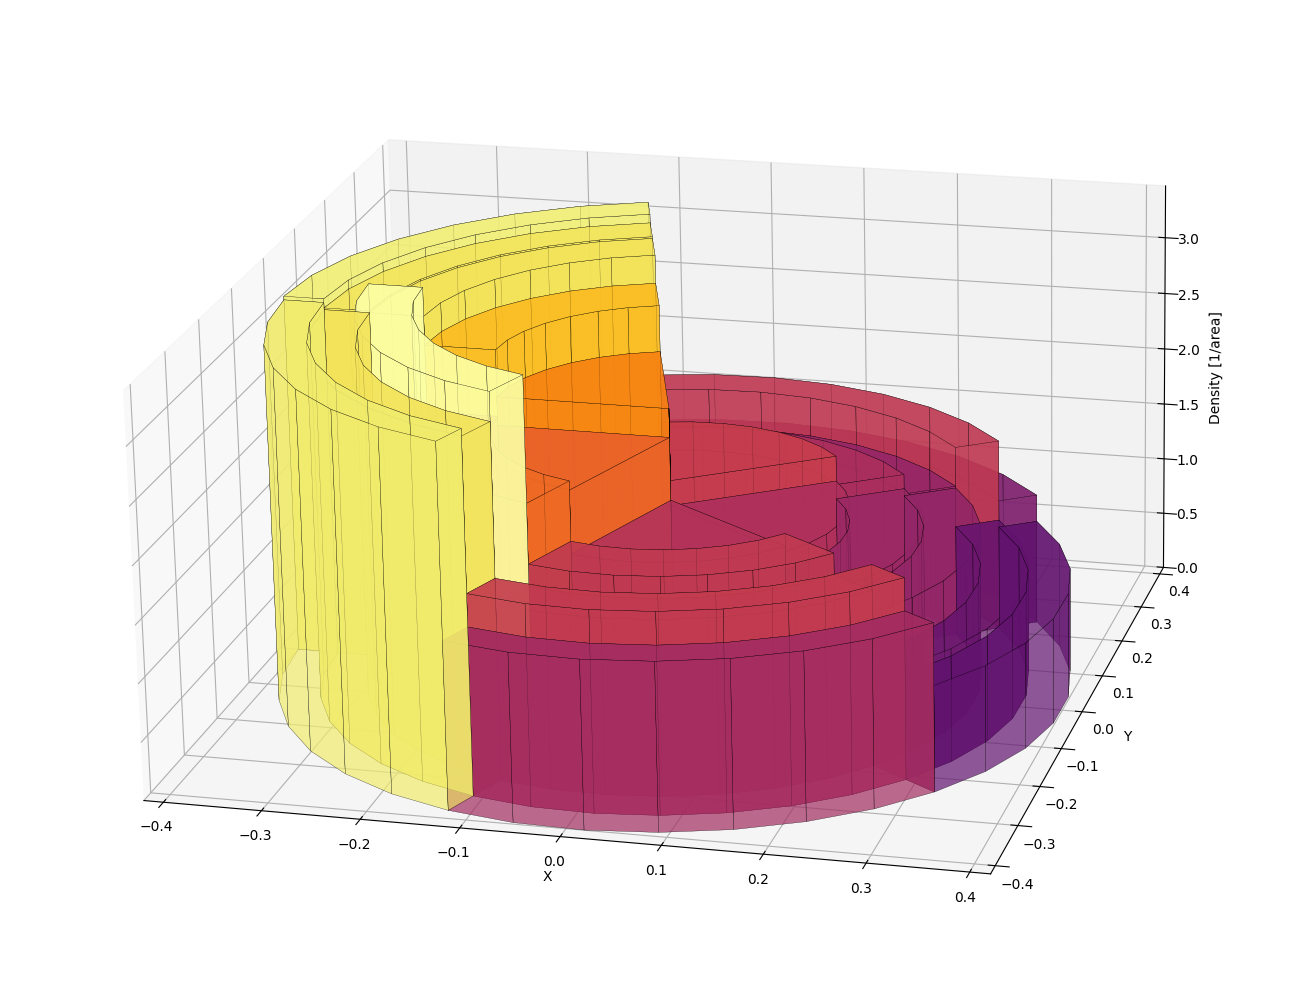
\includegraphics[width=0.49\textwidth]{images/accettanza/example2.2.png}
            \caption{In questo caso osserviamo come la distribuzione sia particolarmente concentrata sul lato del rivelatore più vicino alla sorgente.}
        \end{figure}
        
        \begin{figure}[ht]
            \textbf{Sorgente e rivelatore confrontabili}
            \lstinputlisting[style = mybash]{code/accettanza/bash3.txt}
            \centering
            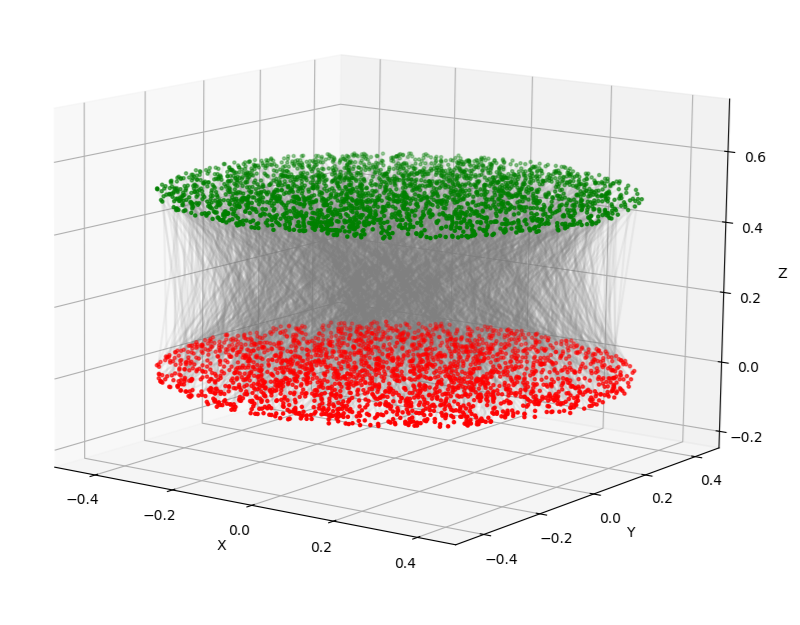
\includegraphics[width=0.49\textwidth]{images/accettanza/example3.1.png}
            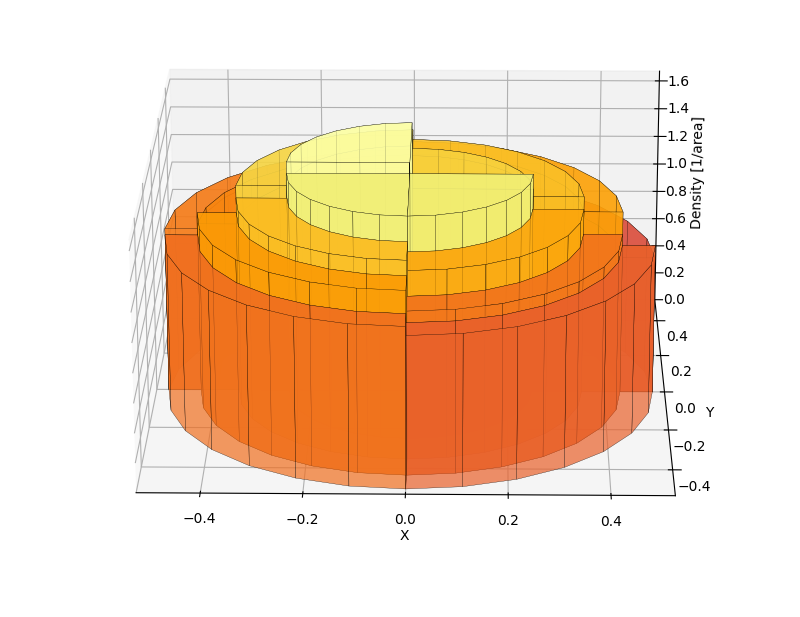
\includegraphics[width=0.49\textwidth]{images/accettanza/example3.2.png}
            \caption{Anche qui come nel primo caso la distribuzione dei raggi è più densa al centro e qualitativamente a simmetria cilindrica.}
        \end{figure}

        \begin{figure}[ht]
            \textbf{Sorgente grande e rivlatore vicino}
            \lstinputlisting[style = mybash]{code/accettanza/bash4.txt}
            \centering
            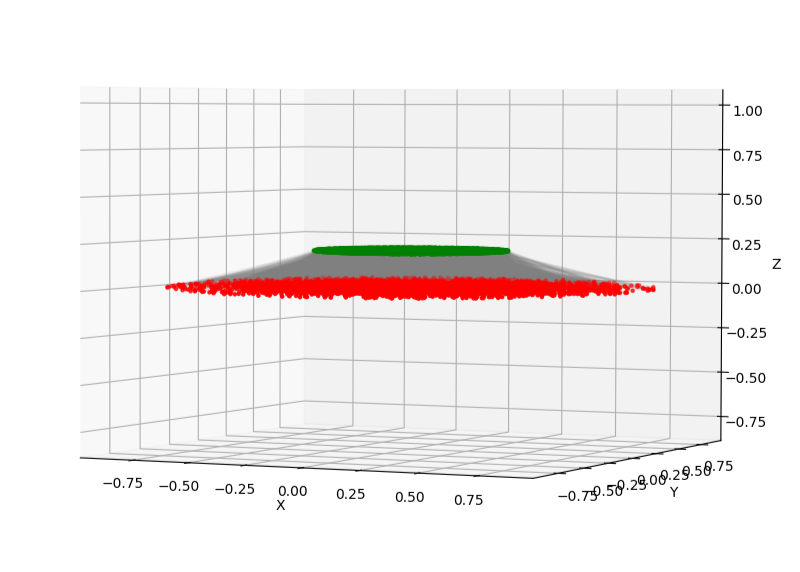
\includegraphics[width=0.49\textwidth]{images/accettanza/example4.1.png}
            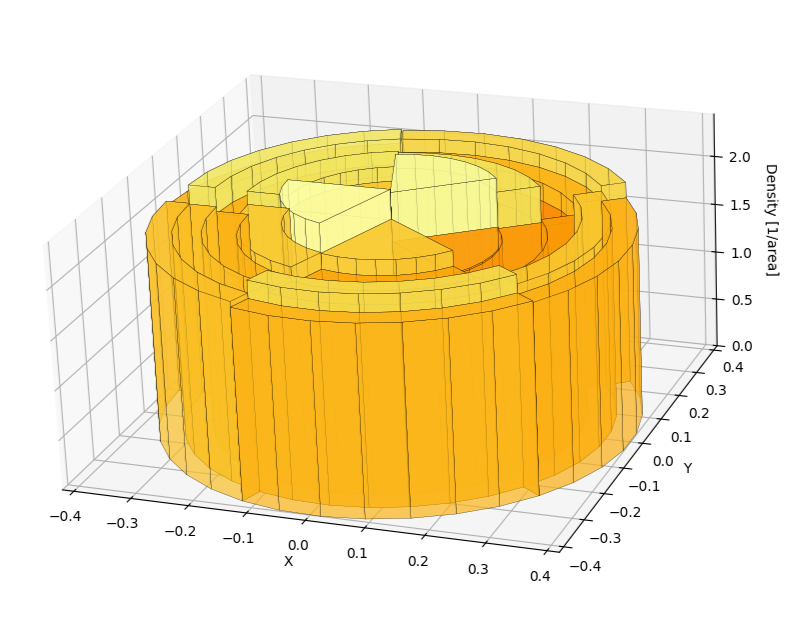
\includegraphics[width=0.49\textwidth]{images/accettanza/example4.2.png}
            \caption{Ponendo un rivelatore piccolo molto vicino alla sorgente la distribuzione appare in prima approssimazione uniforme.}
        \end{figure}

        